% Font size needs to be at least 12-pt.

\documentclass[12pt]{article}
\usepackage[utf8]{inputenc}
\usepackage{amsmath}
\usepackage{amssymb}
%\usepackage[left=1.0in,right=1.0in,top=1.0in,bottom=1.0in,pdftex]{geometry}
\usepackage{fancyhdr}
\usepackage{setspace}
\usepackage{lastpage}
\usepackage{graphicx}
\usepackage{comment}

\fancypagestyle{firststyle}
{
   \fancyhf{}
   \lhead{\textbf{Problem Chosen}\\ \Large{\textbf{Problem A}}}
   \chead{\textbf{2021}\\ \textbf{MCM/ICM}\\ \textbf{Summary Sheet}}
   \rhead{\textbf{Team Control Number}\\ \Large{\textbf{2118048}}}
   %\cfoot{\thepage}
   %\topmargin -0.5in
   \setlength{\headheight}{44pt}
   %\setlength{\footskip}{20pt}
   \renewcommand{\headrulewidth}{2pt}
}

\pagestyle{fancy}
\fancyhf{}
\lhead{Team 2118048} 
\rhead{Page \thepage\ of \pageref{LastPage}}
\cfoot{\thepage}
%\setlength{\headheight}{20pt}

\title{The World is Going to Shiitake: The Effects of Climate Change on Fungi and Decomposition}

\author{Team 2118048}
\date{February 8, 2021}



\begin{document}




\thispagestyle{firststyle}

Fungi possess a wide range of unique abilities and are used in many ways including food, medicine, and spiritual experiences, but perhaps one of their most important roles is not really a ``use'' at all: their natural job as decomposers. By decomposing woody fibers and plant litter, fungi play an important role in the carbon cycle, delivering carbon from dead plant material into the soil where it can be stored.  

Different species of fungi decompose wood and plant litter at different rates. We will be modeling the decomposition rate of plant material by multiple species of fungi based on two of fungal traits. The traits we will be focusing on are hyphal extension (growth) rate and dominance-tolerance trade-off which essentially determines whether a specific fungus prioritizes niche dominance or tolerance to moisture fluctuation. In our model, we explore how the environmental moisture selects for different fungal species and traits. We study the science of climate change and how it impacts fungal communities, taking into account factors such as biodiversity and changing environmental conditions. We also consider how other factors such as temperature, rot type, and wood composition could improve our model. 

Further, we looked more closely at the different species of fungi to determine the relevance of their specific advantages and disadvantages when it comes to decomposition, and what environments in which each fungi might find an ideal home.  

Finally, our article takes a broad look at the ways fungi interact with the environment. We assess the current role of fungi within ecological systems and discuss how that role could change. Fungi will need to adapt to changes within their individual environments as changing temperatures allow for increased biodiversity. As more extreme weather and climate patterns cause increased risk of forest fire, fungi will continue to play an important role in maintaining forests and regulating carbon. 


\newpage 

\setcounter{page}{2}
\maketitle

\vspace{30mm}

\begin{center}
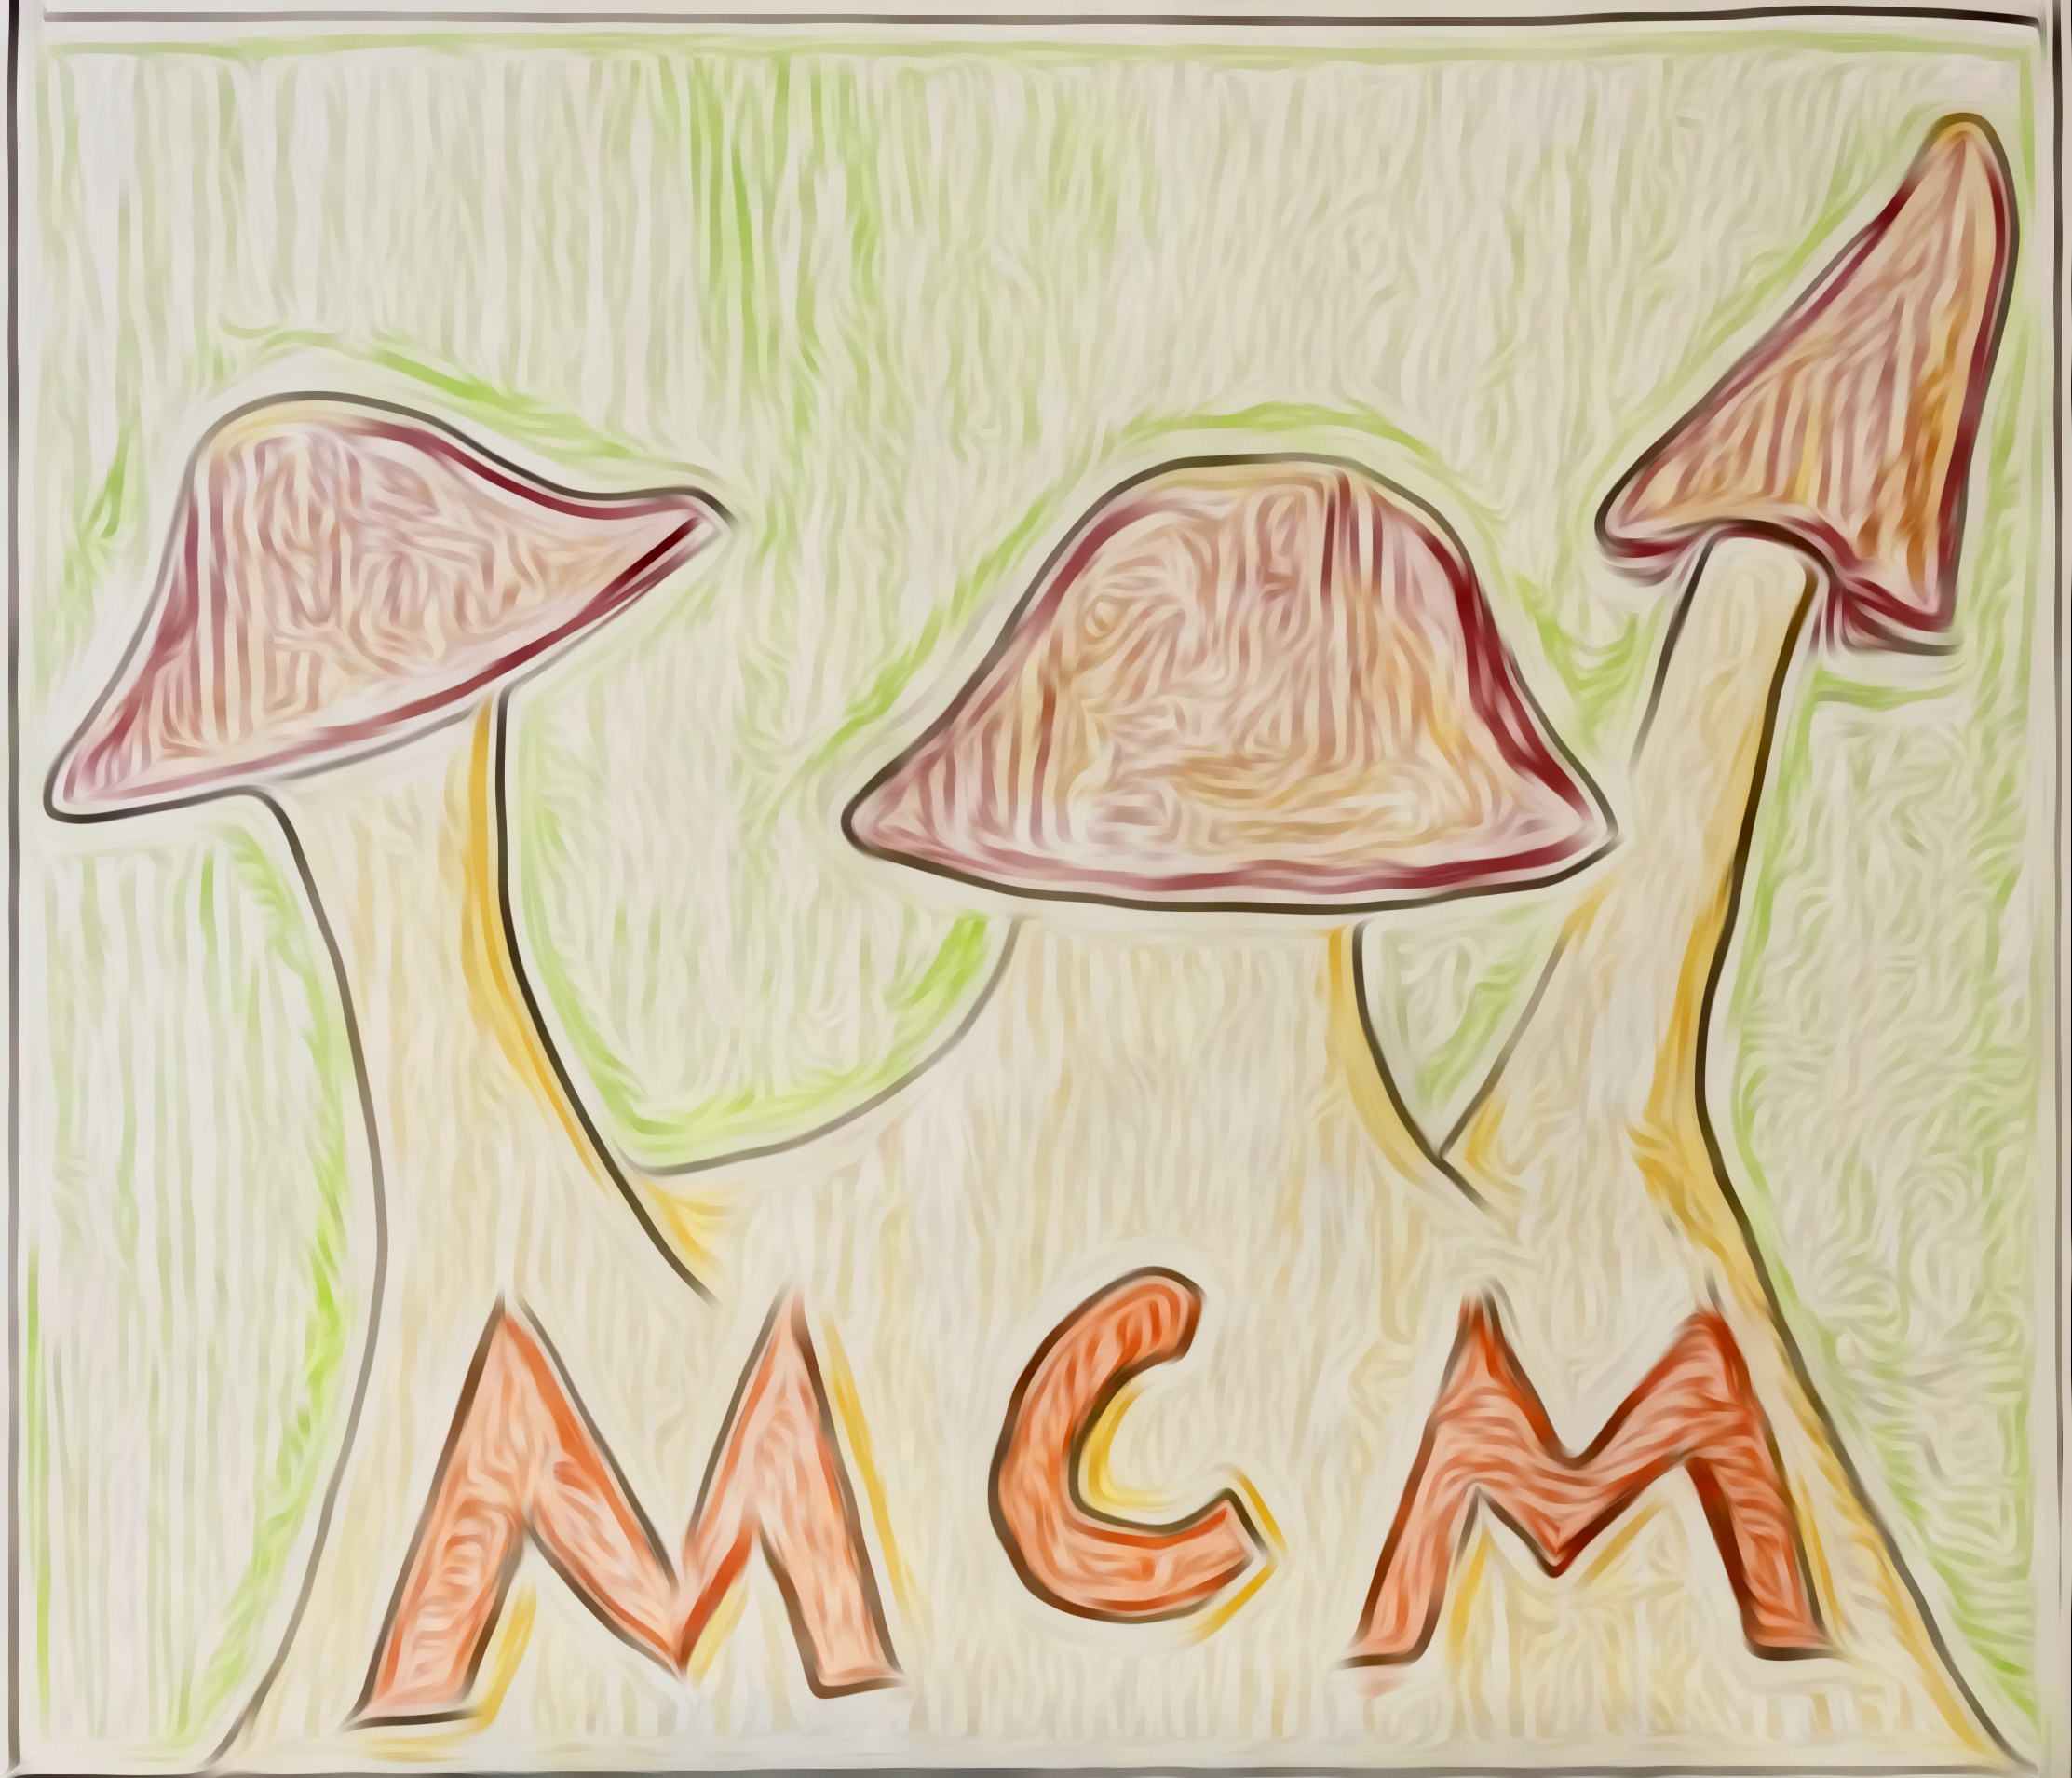
\includegraphics[width=9cm]{MCMushroom.JPEG}
\end{center}

\newpage
\tableofcontents
\newpage

\section{Introduction}

For this model we will be looking at specific fungal traits that impact decomposition rates and modeling the rate of decomposition based on the combined effects of those traits. The two traits we will focus on are hyphal extension rate and dominance-tolerance trade-off. These traits vary across fungal species and are affected by environmental factors such as moisture. We will use data of these variations across eight specific fungi species to find a relation between the environment and the fungi that grow there. From there, we will model how these traits impact decomposition rate and to what extent each of the traits comes into play. Further, because of this relation, we will use our model to look at decomposition rates across a broad range of ecosystems. Of course, no model is perfect so we will also assess the strengths and weaknesses of our model and propose ways the model could be improved.

\begin{center}
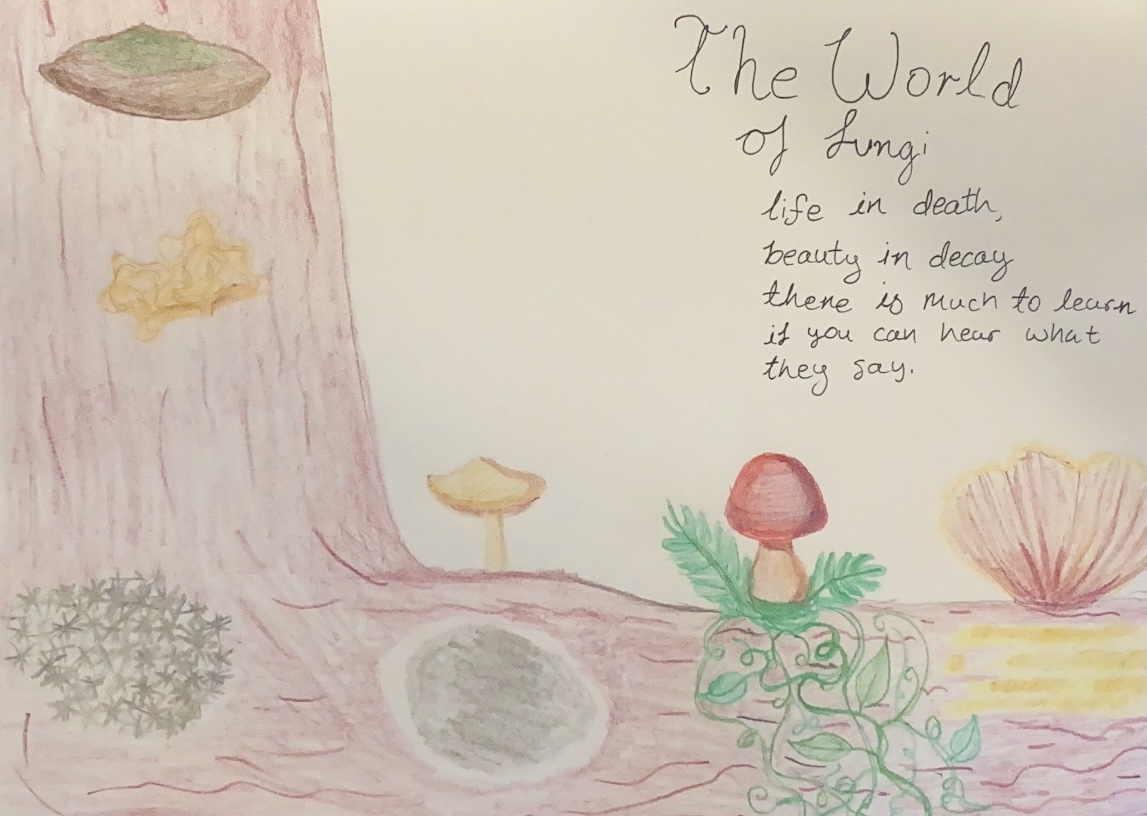
\includegraphics[width=12cm]{sophiaMCM.jpg}
\end{center}


\section{Assumptions}
 
The fungal species modeled have 4 characteristics, which are measured by \cite{source25} decomposition rate, dominance-tolerance trade-off, hyphal extension rate, and optimal moisture. Our model assumes the variation in decomposition rate is determined entirely by the dominance-tolerance trade-off and hyphal extension rate. 

We make the assumption that the average optimal moisture of a fungal community reflects the moisture of its environment. We assume that changes to environmental conditions (an increase or decrease in moisture) will cause the ratio and makeup of species in that community to change over time to exhibit a new average optimal moisture reflective of the new environmental conditions. 
 
% "Optimal moisture" value is assumed to reflect the environmental conditions. That is, we assume that the average optimal moisture of a collection of individuals in a region will reflect exactly the actual moisture conditions. 




\section{Our Model}

The model is
\[
D = 10 \frac{0.19*G^{0.32} + 0.15 * e^{T*0.82+1}}{0.19+0.15},
\]
where $D$ is the decomposition rate (in percent decrease after 122 days from 0-100), $G$ is the hyphal extension rate (in millimeters per day), and $T$ is the dominance-tolerance trade-off (from -1 to 1). 

We also model the relationship between the moisture, growth and trade-off as
\[
T = -1.5 M + 0.9
\]
and 
\[
G = -11.9 M + 10.8,
\]
where $M$ is moisture of the local environment (in mega pascals).


\subsection{Parameters}
In our model, the parameters can be understood as the following:
\begin{itemize}
\item $D$ is the decomposition rate of a fungal species in percent decrease of wood fiber after 122 days. 
\item $G$ is the hyphal extension rate of a fungal species in mm per day. 
\item $T$ is the tolerance-dominance trade off of a fungal species. 
It represents two connected traits of a fungus: its moisture niche width and its competitiveness relative to other fungi. 
Each of the fungi species the researchers in \cite{lustenhouwer} studied falls on a scale from 0 to 1 for these two traits, with 0 being the least characteristic of that trait and 1 being the most characteristic of that trait.
The value of $T$ is then the difference in these two traits, so that a value of $T = -1$ would correspond to an extremely environmentally-resilient fungus who is easily out competed by other species of fungi, while a value of $T = 1$ would correspond to a fungus which drives other species out of a shared environment, but is incapable of growing in all but a few moisture conditions. 
\end{itemize}

\begin{figure}[h!]
\begin{center}
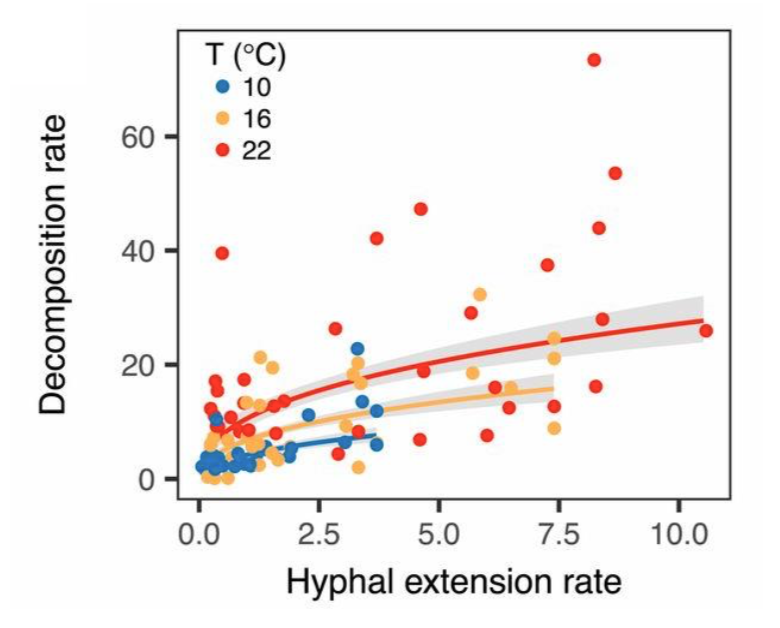
\includegraphics[width=10cm]{GtoD.png}
\caption{A Log-Log Linear Relationship Between the Growth Rate and Rate of Decomposition. Measurements were taken after 122 days across three different temperatures, with all three temperatures exhibiting a similar relationship (Figure 1C in \cite{lustenhouwer}). }
\end{center}
\end{figure}

\begin{figure}[h!]
\begin{center}
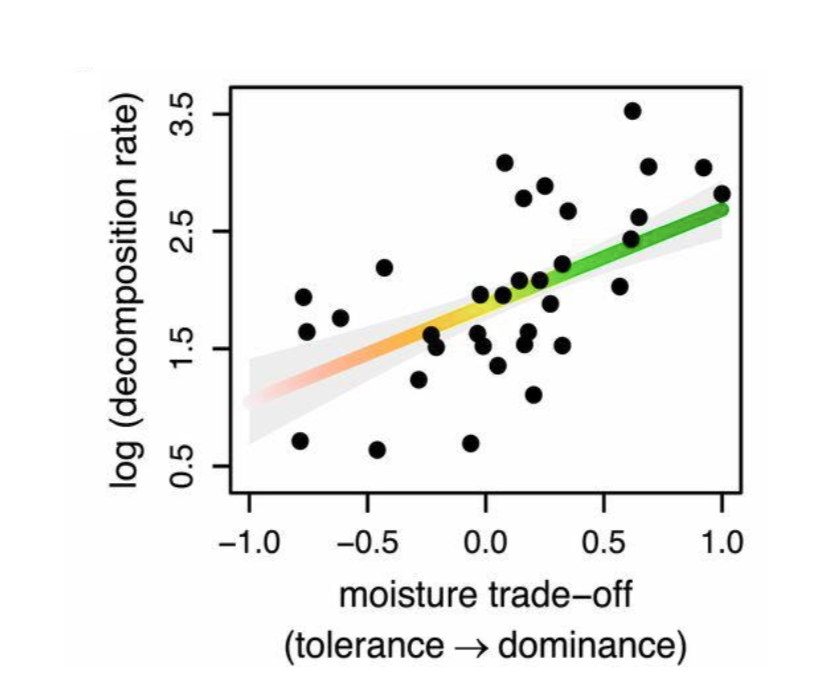
\includegraphics[width=10cm]{TtoD.png}
\caption{A Semi-Log Linear Relationship Between the Tolerance-Dominance Trade-Off and Rate of Decomposition (Figure 4A in \cite{lustenhouwer}).}
\end{center}
\end{figure}

% The contributions of $D(G)$ and $D(T)$ were both included in the determination of $D(T,G)$ through a weighted average. The weights chosen based on the amount of variance accounted for in $D$ determined by the researchers in \cite{lustenhouwer}. 
As shown in \textbf{Figure 1}, Lustenhouwer et al. determined growth rate to account for 19\% of the variance in decomposition rate, with a slope of $0.39$ on a log-log scale.
This gives us the relation 
\[
D(G) = 10*G^{0.39}.
\]
We scale this by a factor of 10 to get a percentage of decomposition after 122 days in an interval consistent with the data. 




As shown in \textbf{Figure 2}, Lustenhouwer et al. determined the dominance-tolerance trade-off to account for some of the variance in decomposition rate, with a slope of $0.82$ and intercept of 1 on a semi-log scale. This gives us the relation
\[
D(T) = 10 e^{T*0.82+1},
\]
again scaled by 10 to get \% decomposition after 122 days. 



The researchers do not specify the amount of variance in $D$ accounted for by the dominance-tolerance trade-off. We know that hyphal extension rate was ``the strongest individual predictor'' \cite{lustenhouwer}  of decomposition rate studied by Lustenhouwer et al., which explained 0.19\% of the variance. Therefore an upper bound on the variance accounted for by $T$ is 0.19. We arbitrarily choose the variance accounted by $T$ to be 0.15, however, the true number could be higher or lower. 

Since both the dominance-tolerance trade-off and hyphal extension rate have been found to predict decomposition rate, we take a weighted average of their relationships. We choose to weight the contributions of each parameter $T$ and $G$ by the variance accounted for by each. This gives us the final model 
\[
D = 10 \frac{0.19*G^{0.32} + 0.15 * e^{T*0.82+1}}{0.19+0.15}. 
\]

\subsection{Bringing Moisture to The Model}


In their study, Maynard et al. measured growth rate, trade-off, and optimal moisture for eight fungal species. We linearly relate growth rate and trade-off each to optimal moisture from their data in 
%Figures number may change
\textbf{Figure 3} and \textbf{Figure 4} shown below. 
%Needs to be updated later
These have the lines of best fit:
\[
T = -1.5 M + 0.9
\]
and 
\[
G = -11.9 M + 10.8.
\]

\begin{figure}[h!]
\begin{center}
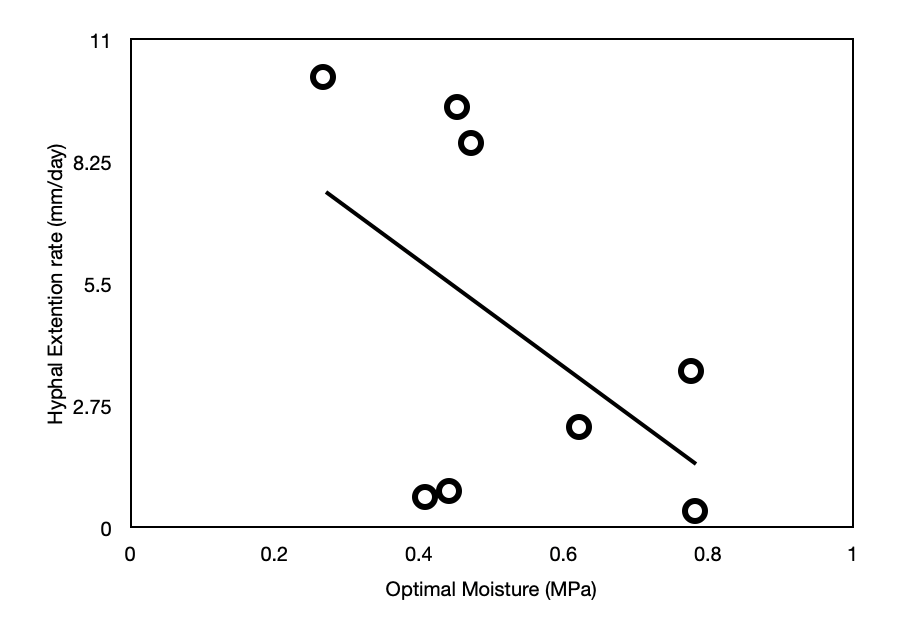
\includegraphics[width=10cm]{MtoG.png}
\caption{A Linear Relationship Between G and M. We assume the local population's average optimal moisture reflects that environment's actual moisture. Data collected by \cite{source25}.}
\end{center}
\end{figure}

\begin{figure}[h!]
\begin{center}
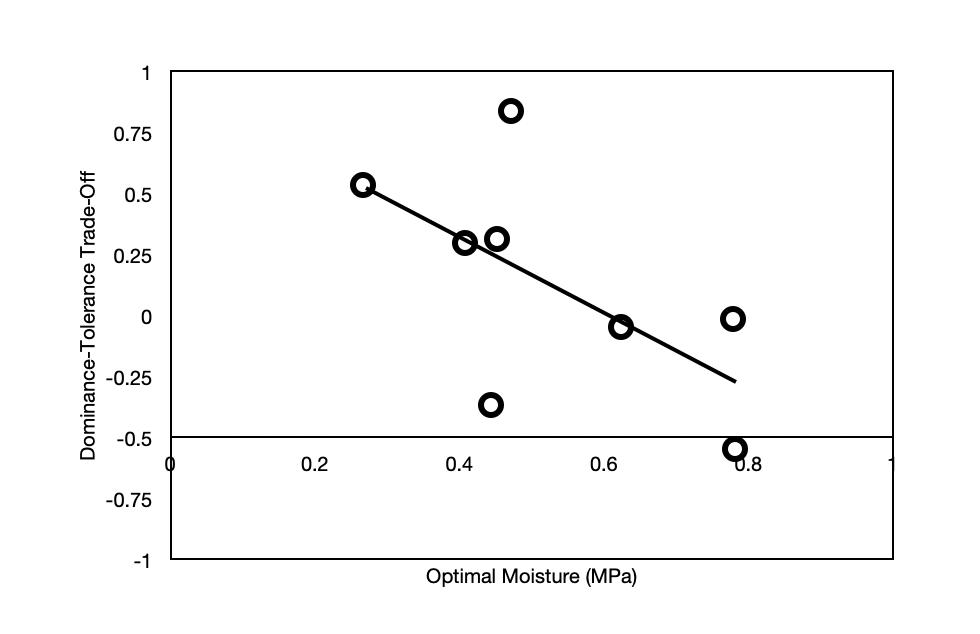
\includegraphics[width=10cm]{MtoT.png}
\caption{A Linear Relationship Between T and M. Data collected by \cite{source25}.}
\end{center}
\end{figure}


% If we think that dominance-tolerance trade-off explains less than \% 15 of the variance in $D$, say \% 10, we will have \[ D =  10 \frac{0.19*(5)^{0.32} + 0.10 * e^{(0.8)*0.82+1}}{0.19+0.10} = 29\%. \] We can see that since this fungus was 

\section{Results and Interpretation}

Our model predicts decomposition rate of a species of fungus based on the growth rate of that fungus and its dominance-tolerance trade-off value. Given a fungus with a hyphal extension rate of 5 millimeters per day, a dominance level of 0.9, and a moisture niche width of 0.1, we calculate 
\[
T = 0.9 - 0.1 = 0.8.
\]
Using the values $T = 0.8$ and $G = 5$ in the model, we predict the percentage of decomposition after 122 days for this fungus to be
\[
D(5,0.8) =  10 \frac{0.19*(5)^{0.32} + 0.15 * e^{(0.8)*0.82+1}}{0.19+0.15}
= 33 \%.
\]

Let's say we are interested in predicting the decomposition rate of a bio-diverse community of fungi, we then first average their growth and trade-off values. Consider we have a collection of 5  Armillaria tabescens individuals and 2 Phlebia rufa individuals, then their (G,T) traits are (0.785,-0.376) and (8.63, 0.832) respectively \cite{source25}. So the average of these two traits for this fungal community is

\[ (G,T) = \frac{5 * (0.785,-0.376) + 2 * (8.63, 0.832)}{7} = (3.026, -0.031). 
\]
Next, we plug our values for $G$ and $T$ into the model to find the average decomposition as
\[
D(3.026, -0.031) = 10 \frac{0.19*(3.026)^{0.32} + 0.15 * e^{(-0.031)*0.82+1}}{0.19+0.15} =  19.6 \%.
\]

Each fungal species referenced in our paper and studied by \cite{source25} has a measured ``optimal moisture.'' This refers to the moisture at which a fungus's growth rate is the highest. Our model makes the crucial assumption that the average optimal moisture of a fungal community reflects the actual moisture that community lives in. Once again considering the community of 5  Armillaria tabescens individuals and 2 Phlebia rufa individuals, we note that Armillaria tabescens have an optimal moisture of 0.445 and Phlebia rufa have an optimal moisture of 0.467 \cite{source25}. So this community has an average optimal moisture of
\[
\frac{5* 0.445+ 2*0.467}{7} = 0.45 \textrm{ MPa}.
\]
From this average optimal moisture, we assume that the actual moisture of the region these mushrooms are located in is 0.45 Mega pascals. If the moisture of that environment subsequently changes, then we predict that the makeup of the fungal community will change so that the optimal moisture more closely reflects the environmental conditions. So, if the moisture went up in this community's region, then we would expect that the optimal moisture would also go up. This would be caused by the ratio of Armillaria tabescens to Phlebia rufa individuals changing, with the number of Phlebia rufa individuals increasing, or the number of Armillaria tabescens individuals decreasing. Our model does not predict how long a change in community make-up will take, on the other hand, only when the change will eventually occur in the long term. Based on this, we cannot predict exactly how short term fluctuations or seasonal differences in climate will cause $G,T$ or $D$ to change, but long term climate change will definitely lead to a change in $G,T$ and $D.$

\begin{center}
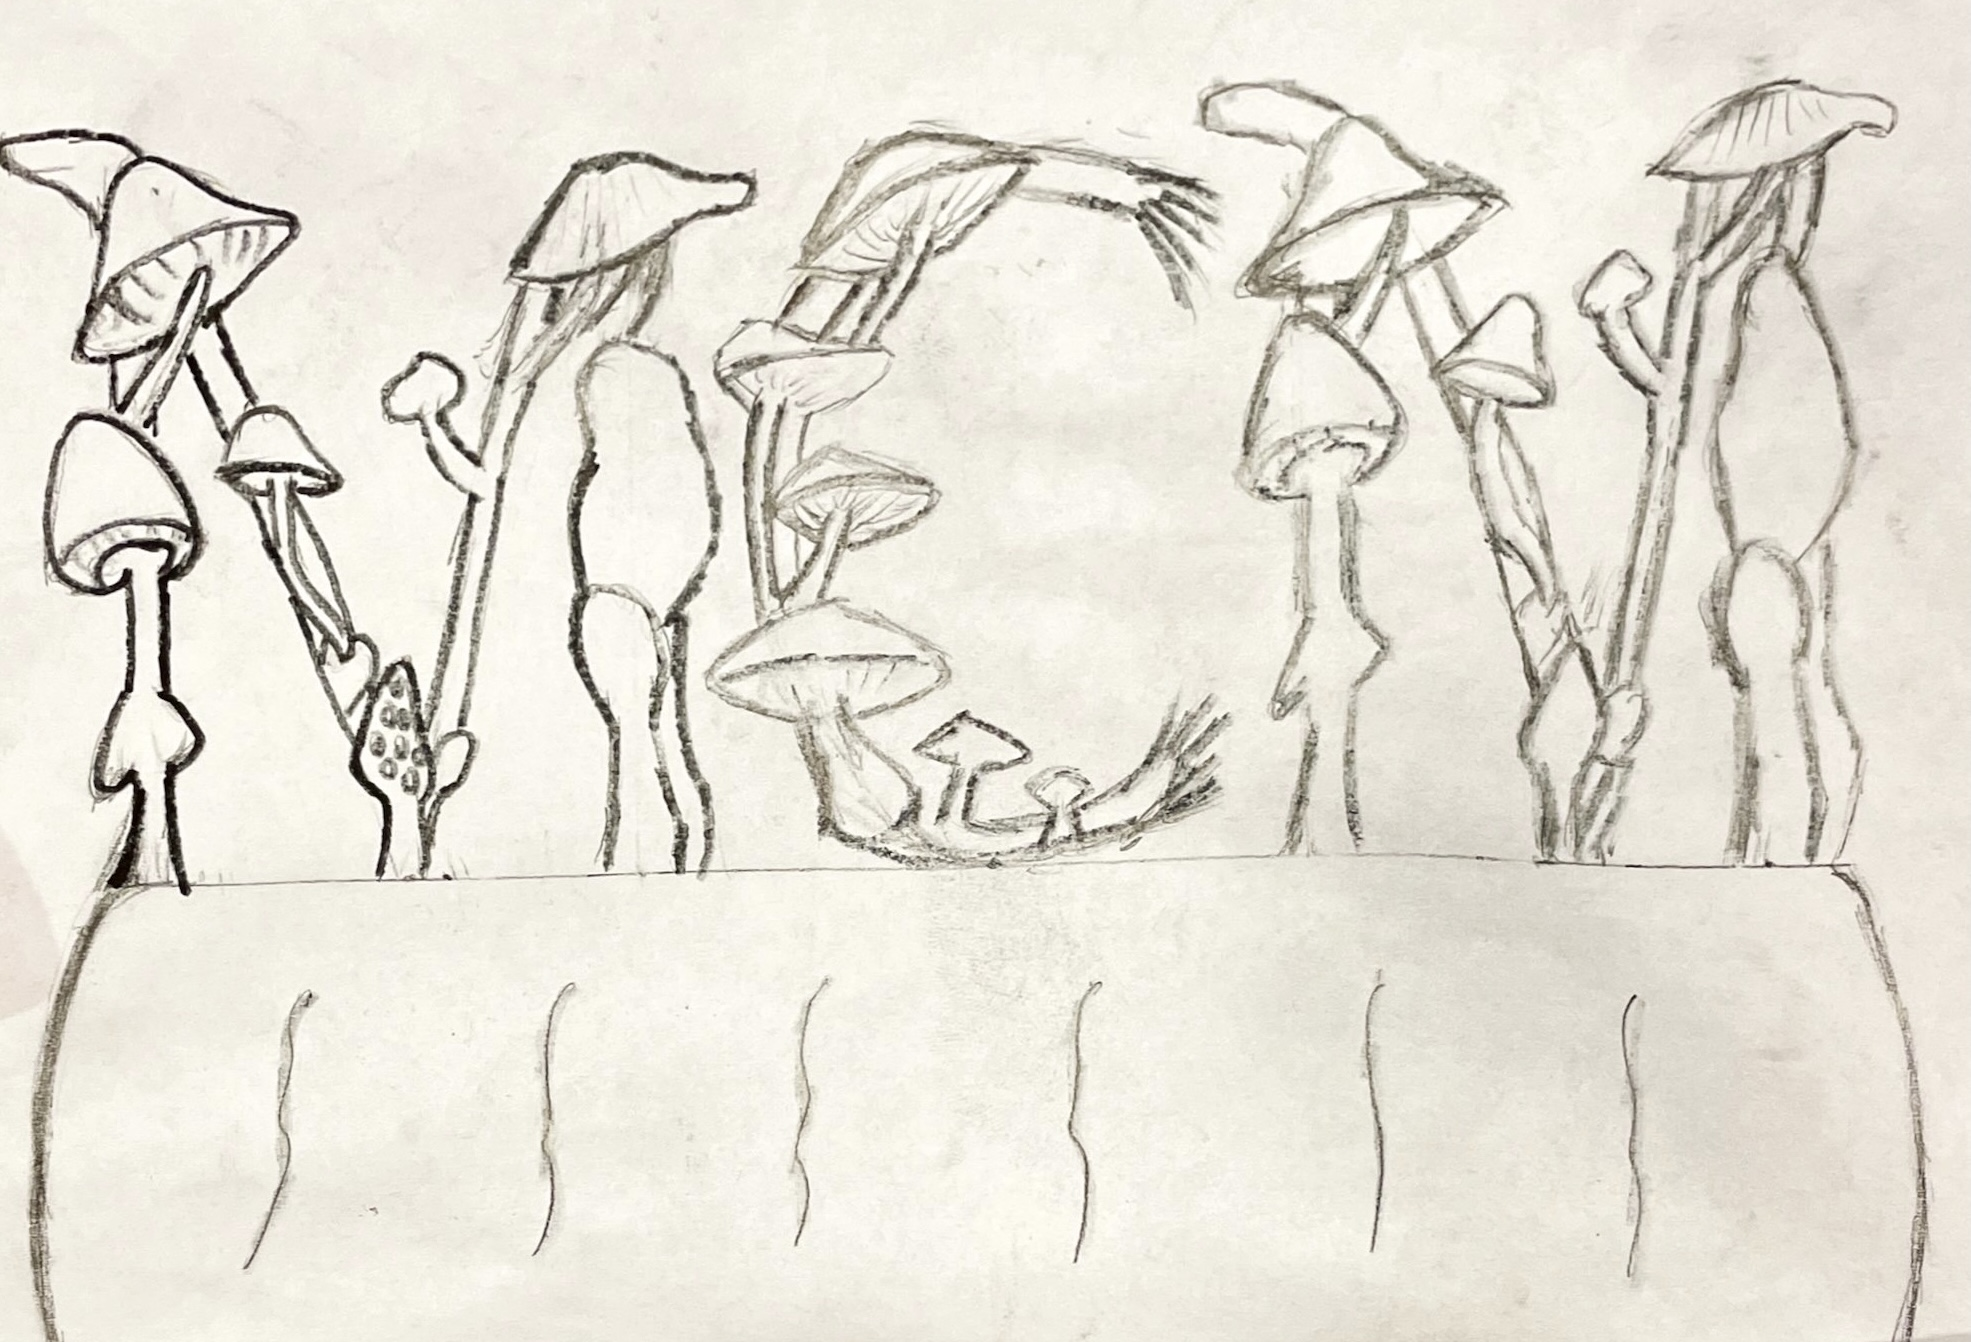
\includegraphics[width=8cm]{tuanmcm.jpg}
\end{center}

\subsection{Five Climates}

We will examine the decomposition rates in arid, semi-arid, temperate, arboreal, and tropical rain forests. These five unique climates represent a spectrum of humidity ranging from least humid (arid) to most humid (tropical). Our model considers the moisture in mega pascals of the environment a fungal community lives in and thus we attempt to relate these five climates to a moisture value considered by our data sources. Of the eight fungal species studied by \cite{source25} and used in our model, the lowest optimal moisture is 0.41 and the highest is 0.78. Therefore, we consider the moisture within that range. We assign arid 0.41 MPa, semi-arid 0.5 MPa, temperate 0.59 MPa, arboreal 0.68 MPa, and tropical rainforest 0.78 MPa. The results from our model for all five of these environments are summarized in
%%%%%
\textbf{Figure 5}. 
%%%%% the table



\begin{figure}[h!]
\begin{center}
\begin{tabular}{|lllll|}
\hline
D (\%) & T     & G (mm/day) & M (MPa) & Climate   \\ \hline
25.0   & 0.285 & 5.921      & 0.41    & Arid      \\
22.8   & 0.15  & 4.85       & 0.5     & Semi-Arid \\
20.7   & 0.015 & 3.779      & 0.59    & Temperate \\
18.6   & -0.12 & 2.708      & 0.68    & Arboreal  \\
16.0   & -0.27 & 1.518      & 0.78    & Tropical  \\ \hline
\end{tabular}
\caption{Our model's predictions for $D,T$ and $G$, given $M.$ $D$ is \% decomposition after 122 days, $T$ is dominance-tolerance trade off, $G$ is growth rate, and $M$ is moisture level. } 
\end{center}
\end{figure}

From our model's results it can be see that as we transition from dry to moist climates, the fungal species found are slower growing and more tolerant of a wider range of moistures.

Global climate change has the effect of making the world moister \cite{moist}. Warm air can hold more water vapor, and so as climate change warms the atmosphere, the humidity will go up. 
If global moisture levels rise by 50\%, our model predicts the rate of decomposition by fungal species will decrease significantly. Previously arid climates could see a drop in decomposition rate by 20\% of their previous value. 
This would be a result of the low moisture niche width but quickly decomposing fungal species being unable to continue their growth in those areas. 
As moisture increases, the fungi with a high optimal moisture but low decomposition rate will take over. 

\section{Strengths and Weaknesses of Our Model}

In order to obtain single values for its parameters, our model considers a diverse fungal community as a single ``average'' species. By taking the average of a population, our model removes much of the information about biodiversity found by counting the individuals in a population. The interactions between different fungi within a community may be more complex than the sum of a few of their characteristics. In this case, only taking the average of a population could be considered a flaw. 

A crucial assumption of our model is that decomposition rate across fungal species is primarily determined by the dominance-tolerance trade off and the hyphal extension rate. One weakness of our model is that none of the numerous other characteristics of fungi are considered in our predictions of decomposition rate. Researchers at the University of Helsinki found that decomposition rate has a strong correlation with the combination of various fungal rot types (brown rot vs. white rot). Furthermore, different types of fungi rot types are more efficient when decomposing different types of plant material which can also impact decomposition rate \cite{newsRX}. While our model uses only two characteristics to predict decomposition rate, its method of doing so (weighted average) is capable of including additional characteristics easily. These may include some other characteristics like temperature and its relationship in the weighted average to other characteristics.

Another simplifying assumption of our model is that the average ``optimal moisture'' of a fungal community will reflect or change to reflect the actual moisture of their environment. This isn't necessarily the case since the average optimal moisture is bounded by the optimal moisture of the specific fungus species present in that community. If the moisture raises too high and there is no combination of fungi in that region which could reflect that optimal moisture, the our model's assumption clearly does not hold. For this reason, we used only numbers in this paper which were within the reasonable bounds of the eight fungal species chosen. Our goal was staying within the extremes of our data points was held for moisture as well as hyphal extension rate and dominance-tolerance trade-off. 


\section{Our Chosen Fungal Species}

Fungi are a diverse group, and the researchers Maynard et al. collected data on many species. Of the numerous species they studied, eight had data on all four parameters in our model - this group of fungi represent the data points in figures 3 and 4. In order to contextualize the data our model is based on, it will be helpful to examine the characteristics of each of these fungal species in terms of their advantages and disadvantages based on climate and ecological role.

\subsection{Hyphoderma setigerum}

\textbf{Hyphoderma setigerum} plays an important role in forest management in Europe. The study in \cite{blackCherry} describes the use of this fungus to gain control over black cherries in Kampinos National Park which run rampant all across Poland. The ability to eliminate invasive species makes \textbf{Hyphoderma setigerum} a good fungal species to live in either temperate or tropical forest conditions.

\begin{figure}[h!]
\begin{center}
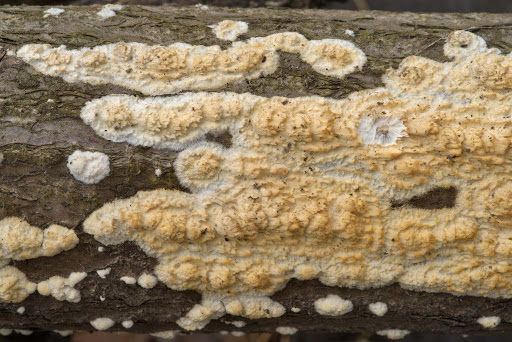
\includegraphics[width=4cm]{Hyphoderma.jpg}
\caption{Hyphoderma setigerum. \centering http://www.asergeev.com/pictures/archives/compress/2017/2006/07.htm }
\end{center}
\end{figure}

%FORMAT HERE UGH
\subsection{Merulius tremellosus}
\textbf{Merulius tremellosus} can be found mostly on decaying logs and stumps in broadleaf forests. In \cite{Merulius}, the advantage of \textbf{Merulius tremellosus} was shown as it can be used on rotten woods to make nutrients for plant soils. Given its characteristics and location, this fungal species will fit in temperate conditions as temperate environment is where broadleaf trees live.

\begin{figure}[h!]
\begin{center}
\includegraphics[width=4cm]{tremellosus.jpg}
\caption{Merulius tremellosus. \centering
https://commons.wikimedia.org/wiki/Merulius tremellosus}
\end{center}
\end{figure}

\subsection{Phlebia rufa}

This fungus shares most of its characteristics with the rest Phlebia genus \cite{Phlebia}. Interestingly, in North America, this fungus is only known to Washington state, Oregon, and British Columbia \cite{Phlebia2}. based on these locations, they also imply that \textbf{Phlebia rufa} is from a more temperate and arboreal environment. 

\begin{figure}[h!]
\begin{center}
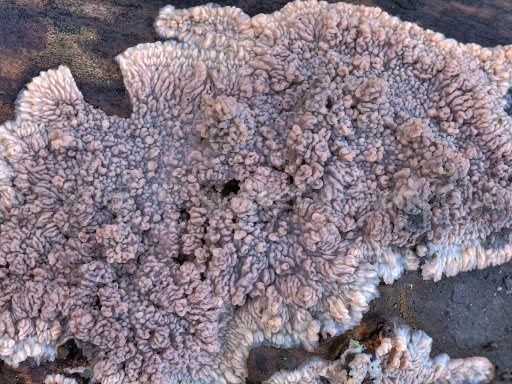
\includegraphics[width=4cm]{rufa.jpg}
\caption{Phlebia rufa. \centering
http://www.rakm.co.uk/fungi\_pages/phlebia\_rufa\_02.htm}
\end{center}
\end{figure}

%MORE FORMAT WORK
\subsection{Phlebiopsis flavidoalba}
\textbf{Phlebiopsis flavidoalba} is another fungus that plays a significant role in its fungal families, specifically Phlebiopsis. While this fungus is not as well known as its family member \textit{gigantea}, it is currently one of the most competitive fungi on Earth. Due to its competitiveness, we believe that this fungi will mostly present more in arid or semi-arid environments.

\begin{figure}[h!]
\begin{center}
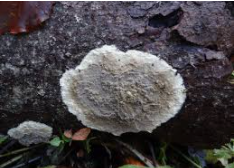
\includegraphics[width=4cm]{phlebio.png}
\caption{Phlebiopsis. \\ https://en.wikipedia.org/wiki/Phlebiopsis}
\end{center}
\end{figure}


\subsection{Schizophyllum commune}
A more well known fungus, \textbf{Schizophyllum commune}, can be found in rainy areas. Like \textbf{Hyphoderma setigerum}, this fungus is also attracted to fruit bearing plants. \textbf{Schizophyllum commune} is beneficial to natural environments but also has medicinal properties and culinary uses \cite{Spitgill}. \textbf{Schizophyllum commune} prefers areas with lots of moisture which would make it a slow growing fungal species living in arboreal or tropical forest areas. 

\begin{figure}[h!]
\begin{center}
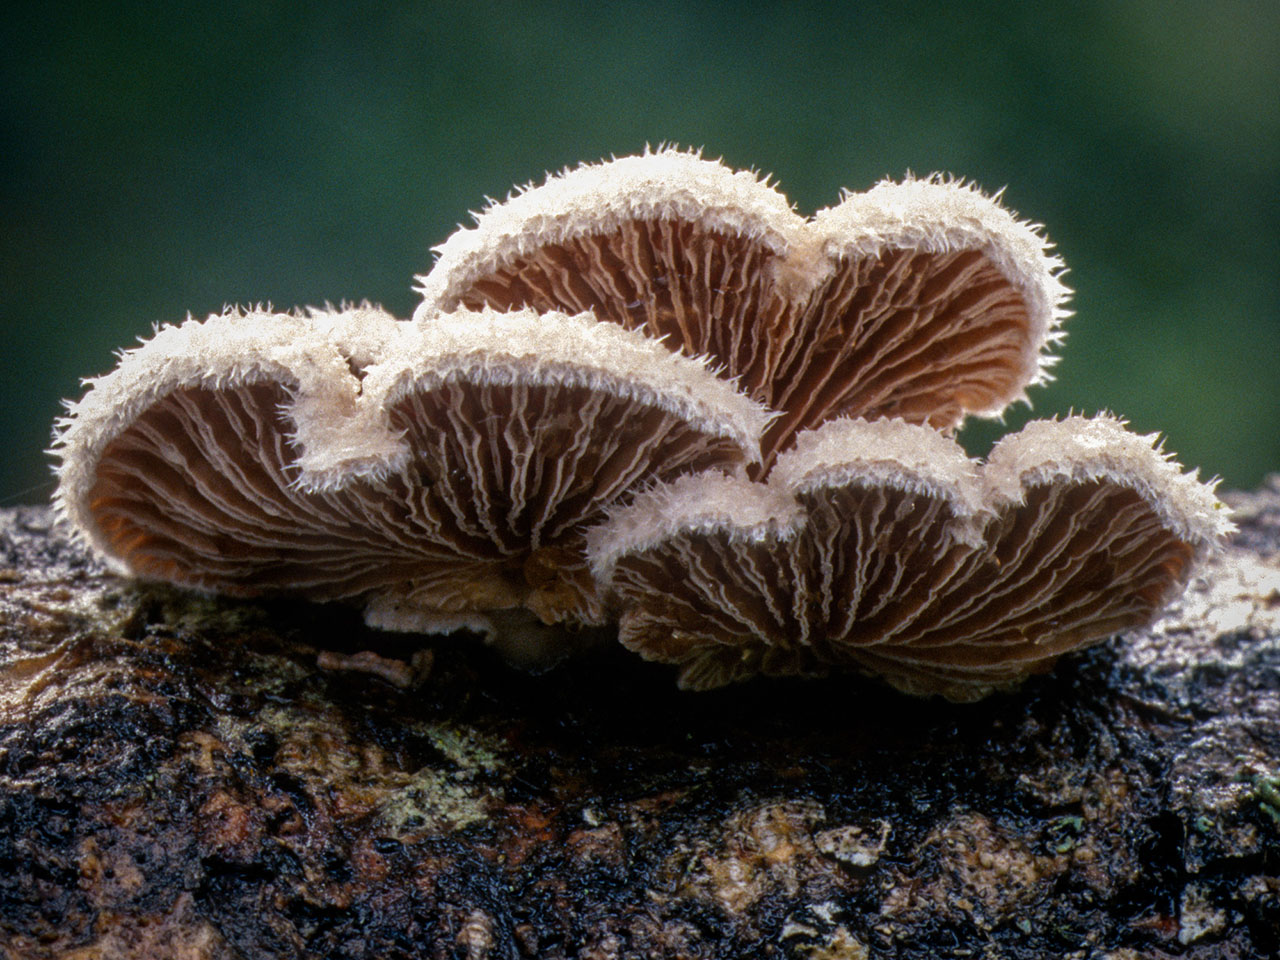
\includegraphics[width=4cm]{spitGill.jpg}
\caption{Schizophyllum commune. \centering https://www.mykoweb.com/CAF/species/Schizophyllum\_commune.html}
\end{center}
\end{figure}

%formattttttttttt
\subsection{Armillaria tabescens}
Unlike other fungi, \textbf{Armillaria tabescens} has a wide range of habitat, it can be found in the Eastern US but also in the Midwest. This type of fungus grows on hardwoods and conifers. This fungus acts as a pathogen that actually kills bark and cambium and roots on stressed trees rather than decaying the root system like other fungi. Similarly to \textbf{Schizophyllum commune}, \textbf{Armillaria tabescens} is also edible for humans \cite{armill}. This fungus typically fruits from summer to fall time which indicates that it would be more suitable for a wide range of environmental conditions. 


\begin{figure}[h!]
\begin{center}
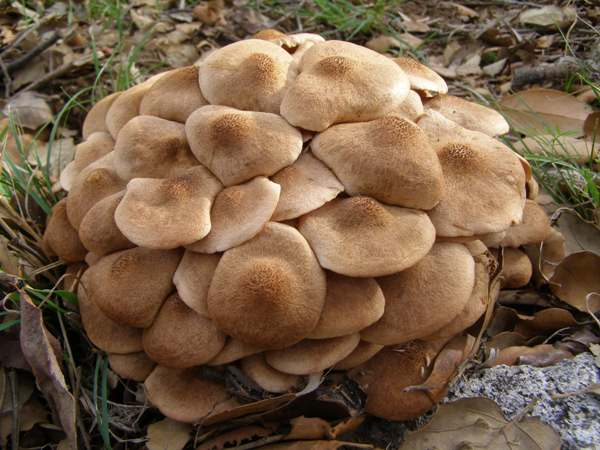
\includegraphics[width=4cm]{honeyFun.jpg}
\caption{Armillaria tabescens. \centering https://www.first-nature.com/fungi/armillaria-tabescens.php}
\end{center}
\end{figure}

\subsection{Armillaria gallica}
\textbf{Armillaria gallica} is another fungus that can also be found in the forest of mixed hardwoods and conifers. This wood-decay fungus is common and ecologically important. It usually lives as a saprobe on logs or weakened trees. Due to its similarities to \textbf{Armillaria tabescens}, this fungus would also be tolerant to a wide range of environments.

\begin{figure}[h!]
\begin{center}
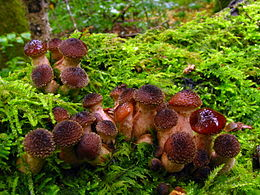
\includegraphics[width=4cm]{gallica.jpg}
\caption{Armillaria gallica. \centering https://en.wikipedia.org/wiki/Armillaria\_gallica}
\end{center}
\end{figure}

\subsection{Phellinus robiniae}
This fugus can be found wherever black locust trees (and other closely related trees) are common. \textbf{Phellinus robiniae} lives on the heartwood of living trees or on the sap of dead woods \cite{robin}. Since this fungus usually spots on dry trees, it is best to consider it in a more arid or semi-arid environments. 

\begin{figure}[h!]
\begin{center}
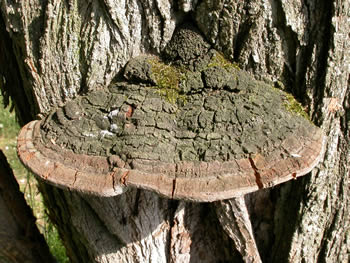
\includegraphics[width=4cm]{robin.jpg}
\caption{Phellinus robiniae. \centering 
https://www.messiah.edu/Oakes/Phellinus robiniae}
\end{center}
\end{figure}




% \section{Our Predictions}
% Given our model and the traits for all eight fungal species above, we predict that fungal species that shared the same environmental conditions will likely survive longer together. Our predictions can be understood as follow:
% \begin{itemize}
   % \item \textbf{arid}: Phlebiopsis flavidoalba, Armillaria tabescens, Armillaria gallica, Phellinus robiniae.
    % \item \textbf{semi-arid}: Phlebiopsis flavidoalba, Armillaria tabescens, Armillaria gallica, Phellinus robiniae. 
    % \item \textbf{temperate}: Hyphoderma setigerum, Merulius tremellosus, Phlebia rufa.
   % \item \textbf{arboreal}: Phlebia rufa, Schizophyllum commune.
   % \item \textbf{tropical rain forests}: Hyphoderma setigerum, Schizophyllum commune.
% \end{itemize}

\section{Model Improvements}

Our model makes predictions about which type of species are most numerous depending on area, and shows how differences in moisture might effect different fungi. In the wetter areas, the majority of the fungi will be ones with negative dominance-tolerance trade-off values such as those in the Armillaria genus. However, in the dryer areas (when there is also a greater abundance of ground litter), the primary fungi will likely be ones with positive dominance-tolerance trade-off values such as Phlebia rufa and Merulius tremellosus. 

Under consistent weather conditions, fungal biodiversity will be rather low, as one species tends to edge out the other \cite{Toljander}. However, with the advent of climate change and more rapid and extreme temperature fluctuations, biodiversity of fungal species has become more possible. To include this in our model, we would need a better understanding of how fungi interact with the environment and each other. We would primarily need to look at how fungi react to temperature fluctuations as that is the condition that seems to relax their competitive tendencies. 

Our model treats different combinations of fungi as an average of their individual characteristics in just two numbers ($G$ and $T$). We must consider what is lost by labeling our fungi in such a reductive way. As we have shown in the previous section, there is significant variation in ecological niche within just these eight species. Many of the fungi grow on different trees, yet our model did not account for wood type in its predictions of decomposition rate. Lustenhouwer et al. determined that after three years, wood type accounted for a staggering 57\% of the variation in decomposition, while hyphal extentsion rate accounted for only 27\%. Based on our knowledge of these eight fungi and Lustenhouwer et al.'s findings, we suggest the model could be improved by including a parameter to account for wood composition. 

%The model might be improved by incorporating error bars around its predictions and parameters. Since most of the model was pulled from the analysis by \cite{lustenhouwer} rather than our own examination of the data, we we not able to include a detailed examination of variance's role in our model. Well explained error bars would make a good inclusion to the model. Pulling from the data directly would also have allowed us to use more accurate numbers for the weighted average of the growth rate and the dominance-tolerance trade-off. 
% ^ Removed this section since it doesn't fit anywhere. ^

\section{Conclusion}

Our model makes the assumption that decomposition rate is determined by hyphal extension rate and dominance-tolerance trade off. The model assumes that a fungal community's average optimal moisture conditions will either represent or change to represent the physical moisture conditions of their environment. Based on the results from the data in \cite{lustenhouwer,source25}, we model the relationship between decomposition rate (D), growth rate (G), and dominance-tolerance trade-off (T) as 
\[
D = 10 \frac{0.19*G^{0.32} + 0.15 * e^{T*0.82+1}}{0.19+0.15}.
\]
Our model predicts that fungal populations with high average growth rate or high dominance will decompose at a faster rate, while fungal populations which are more resistant to the effects of climate change will decompose at a slower rate. 

Based off of our own analysis of the data in \cite{source25} we model the relationship between moisture (M), growth rate (G), and dominance-tolerance trade-off (T) as 
\[
T = -1.5 M + 0.9
\]
and 
\[
G = -11.9 M + 10.8.
\]

We use eight fungi to make this relation of moisture to growth rate and trade-off, and we give a brief biography of each fungi. It is evident that these 8 fungi form a bio-diverse cross section of the wood decomposing fungal kingdom. 

With these relations, our model predicts that as moisture increases globally due to climate change, decomposition rates will decrease across arid to tropical climates - leaving more burnable wood fiber across forest floors. This means (somewhat paradoxically) that as the air gets wetter the chance of forest fire will increase. 

\section{Article: The Role of Fungi in Ecological Systems as The Climate Changes}

Fungi play an important role in the worlds carbon cycle because the woody fiber and plant litter that fungi decompose is mostly of carbon. Through the process of decomposition, carbon is either stored in the soil or emitted into the atmosphere \cite{voriskova}. 
However, because fungi play such an important roll, their traits also have serious effects on ecosystems, environments, and even climate change. In fact, plant litters may contribute as much as 16 percent of the carbon emissions from the earth's soil. Climate change and increase in temperatures is also increasing humidity across the globe. These changes effect fungi directly and make fungal populations more biodiverse as the quality of plant litter available to them changes \cite{ivanov}. Decomposition rates are highest with an intermediate level of biodiversity, but lower biodiversity leads to the highest metabolic efficiency \cite{Toljander}. Globally changing conditions in temperature allow for more biodiversity of decomposing fungi in one environment. 

The competition between fungal species also impacts biodiversity \cite{Toljander}. In fact, the competition between fungal species is perhaps the most important interaction between species. With two or more species in play, one species tends to completely take over the others and this results in relatively low biodiversity. When conditions fluctuate rapidly however, these competitive behaviors seem to relax - allowing for greater species richness \cite{Toljander}. However, that richness will likely have a higher concentration of fungi with negative dominance/tolerance trade-off trait values as increased moisture will work against fungi with higher values. In places with relatively consistent environmental conditions, we can expect low levels of fungal biodiversity, and, depending on the environment, the fungi with higher dominance/tolerance trade-off values will dominate in such areas. 

Feedback loops occur the effect of a single phenomenon leads to more phenomena that in turn lead to more of the original effect. The effect of fungi on the environment and climate change is one example of a natural feedback loop. 
The effects of climate change include higher moisture which, based on our model, effects the actual community make-up of fungi decomposing plant litter. More specifically, as moisture increases, our model indicates that the composition of fungal organisms will be dominated by slow growing, slow decomposing species of fungi that have more robust defenses against changing conditions. This means that the process of fungal decomposition will be significantly slowed and the process of carbon transfer from plant litter to the soil and from soil to the air will be altered as well. Since we have never seen these kinds of changes before, it’s difficult to predict how this will effect the feedback loop. The extended time it will take for woody fibers and plant litter to decompose also allows more time for other environmental processes to take place, such as wildfires. This would mean that the carbon in the burned plant litter would be going directly into the atmosphere, with none of it being stored in the soil. 

Events such as fire are also becoming more frequent and intense as a result of climate change. Fires specifically play an important role in shaping the biochemistry of ecosystems by changing the levels of carbon and nitrogen stored in the soil \cite{pellegrini}. With more frequent fires, these altered chemical levels in the soil become more pronounced and pervasive. Fires reduce carbon inputs into soil through plant litter, and decrease the overall amount of plant litter as well as the amount of fungi in the places they affect \cite{pellegrini}. Further, frequent and high intensity fires can lead to an overall change in the composition of fungal species at play in a given forest when fungi that are destroyed by fire are replaced by opportunist species. Fire also reduces nitrogen levels in the soil, which limits the amount of nitrogen available for plant and fungal life \cite{pellegrini}. All of these effects have subsequent effects on decomposition. In the grand scheme of things, nothing is certain and it is often hard to make predictions based on the unprecedented phenomena that are so common when it comes to the effects of climate change. However, the unique qualities of fungi have many scientists and researchers hopeful that fungi will play an important roll in finding solutions to big environmental problems. 




\newpage

\section{References}
\renewcommand\refname{}

\begin{thebibliography}{9}

\bibitem{lustenhouwer}
Nicky Lustenhouwer, Daniel S. Maynard, Mark A. Bradford, Daniel L. Lindner, Brad Oberle, Amy E. Zanne, and Thomas W. Crowther.
``A trait-based understanding of wood decomposition by fungi." Proceedings of the National Academy of Sciences of the United States, May 13, 2020. www.pnas.org/content/pnas/117/21/11551.full.pdf

\bibitem{frost}
Frost, Jim. 
``Using Log-Log Plots to Determine Whether Size Matters."  statisticsbyjim.com 

\bibitem{wikipedia}
Wikipedia. 2021. ``Semi-log plot.'' 

\bibitem{armill}
\emph{Wood Decay Fungi of Living Trees}\\
https://www.treerot.com/fungi/armillaria-tabescens/

\bibitem{robin}
Kuo
\emph{Phellinus robiniae}\\
https://www.mushroomexpert.com/phellinus\_robiniae.html


\bibitem{Yale}
\emph{Gladiator games: In the natural world, biodiversity can offer protection to weaker species}
May 15, 2017\\
https://phys.org/news/2017-05-gladiator-games-natural-world-biodiversity.html

\bibitem{Spitgill}
http://wildedibles.teriin.org/index.php?album=Mushrooms/Schizophyllum-commune

\bibitem{Hypho}
Lynne Boddy
\emph{Fungi, Ecosystems, and Global Change}\\https://www.overleaf.com/project/601df052c7daf34e33f2b0af
3rd ed., 2016.
https://www.sciencedirect.com/topics/agricultural-and-biological-sciences/hyphoderma

\bibitem{Hypho2}
Yurchenko, Wu
\emph{Hyphoderma pinicola sp. nov. of H. setigerum complex (Basidiomycota) from Yunnan, China}
Oct.9 2014.
https://www.ncbi.nlm.nih.gov/pmc/articles/PMC5430344/

\bibitem{Merulius}
Blanchette, Reid
\emph{Ultrastructural Aspects of Wood Delignification \\by Phlebia (MeArulius) tremellosus}\\
https://www.researchgate.net/publication/7423221
\_Ultrastructural\_Aspects\_of\_Wood\_Delignification\_by\_Phlebia\_Merulius\_tremellosus

\bibitem{Phlebia}
\emph{Lignocellulose-converting enzyme activity profiles correlate with molecular systematics and phylogeny grouping in the incoherent genus Phlebia (Polyporales, Basidiomycota)}
Oct. 2019
https://www.ncbi.nlm.nih.gov/pmc/articles/PMC4610053/

\bibitem{Phlebia2}
Nakasone, Sytsma
\emph{BIOSYSTEMATIC STUDIES ON PHLEBIA ACERINA,P. RUFA, AND P. RADIATA IN NORTH AMERICA }
https://www.fpl.fs.fed.us/documnts/pdf1993/nakas93a.pdf

% [25]
% https://search.proquest.com/docview/2242103228?pq-origsite=primo

\bibitem{blackCherry}
Marciszewska, Szczepkowski, Otreba
\emph{Black cherry (Prunus serotina Ehrh.) colonization
by macrofungi in the fourth season of its decline due
to different control measures in the Kampinos National Park}
Vol. 62 (2), 78-87

\bibitem{moist}
Willett, Dunn, Kennedy, Berry. (2020) Development of the HadISDH.marine humidity climate monitoring dataset, Earth System Science Data, doi:10.5194/essd-12-2853-2020

 \bibitem{source25}
 Maynard, Daniel S, Bradford, Mark A, Covey, Kristofer R, Lindner, Daniel, Glaeser, Jessie, Talbert, Douglas A, Tinker, Paul Joshua, Walker, Donald M, and Crowther, Thomas W. 
 \emph{Consistent trade-offs in fungal trait expression across broad spatial scales}
 Nature Microbiology, 2019.

\bibitem{ivanov}
Ivanov, A. V.
\emph{Forest Litters as a Link in the Carbon Cycle in Coniferous–Broadleaved Forests of the Southern Far East of Russia}
Eurasian Soil Science, 2018.

\bibitem{newsRX}
NewsRX.
\emph{Study Findings on Microbiology and Ecology Are Outlined in Reports from University of Helsinki (Decomposition of spruce wood and release of volatile organic compounds depend on decay type, fungal interactions and enzyme production patterns)}
Ecology, Environment and Conservation. September 27, 201

\bibitem{pellegrini}
Pellegrini, A. F. A., Hobbie, S. E., Reich, P. B., Jumpponen, A., Brookshire, E. N. J., Caprio, A. C., Coetsee, C., and Jackson, R. B.
\emph{Repeated fire shifts carbon and nitrogen cycling by changing plant inputs and soil decomposition across ecosystems.}
Ecological Monographs, 2020.

\bibitem{Toljander}
Toljander, Y.K., Lindahl, B.D., Holmer, L.
\emph{Environmental fluctuations facilitate species co-existence and increase decomposition in communities of wood decay fungi.}
Oecologia, 2006.

\bibitem{voriskova}
Voříšková, J., Brabcová, V., Cajthaml, T. and Baldrian, P. 
\emph{easonal dynamics of fungal communities in a temperate oak forest soil}
New Phytol, 2014.


\end{thebibliography}{}

\end{document}

